\documentclass[tikz,border=6pt]{standalone}
\usepackage{amsmath,amssymb}
\begin{document}
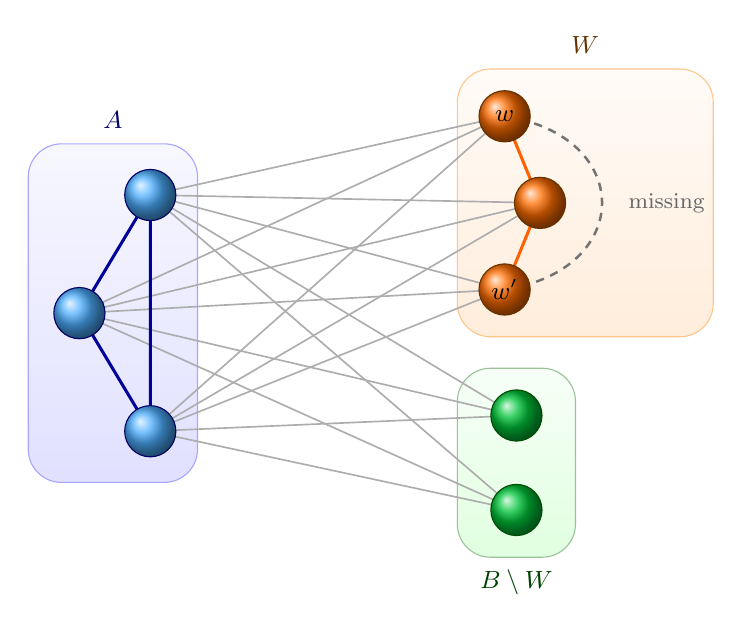
\begin{tikzpicture}[
  av/.style={circle,shading=ball,ball color=blue!45!cyan!70,draw=blue!40!black,minimum size=6.5mm,inner sep=0pt,font=\small},
  wv/.style={circle,shading=ball,ball color=orange!85!red,draw=orange!40!black,minimum size=6.5mm,inner sep=0pt,font=\small},
  bv/.style={circle,shading=ball,ball color=green!55!teal,draw=green!30!black,minimum size=6.5mm,inner sep=0pt,font=\small},
  ae/.style={draw=blue!60!black,line width=1.1pt},
  we/.style={draw=orange!75!red,line width=1.1pt},
  xe/.style={draw=black!32,line width=0.6pt},
  me/.style={draw=black!55,line width=0.9pt,dash pattern=on 3pt off 2.5pt}]
  % panels
  \shade[rounded corners=12pt,top color=blue!3,bottom color=blue!12,draw=blue!35] (-1.55,-0.45) rectangle (0.6,3.85);
  \shade[rounded corners=12pt,top color=orange!3,bottom color=orange!14,draw=orange!45] (3.9,1.4) rectangle (7.15,4.8);
  \shade[rounded corners=12pt,top color=green!3,bottom color=green!12,draw=green!40!black!40] (3.9,-1.4) rectangle (5.4,1.0);
  \node[font=\small,blue!40!black] at (-0.475,4.15) {$A$};
  \node[font=\small,orange!40!black] at (5.525,5.1) {$W$};
  \node[font=\small,green!25!black] at (4.65,-1.72) {$B\setminus W$};
  % vertices
  \coordinate (a1) at (0,3.2);
  \coordinate (a2) at (-0.9,1.7);
  \coordinate (a3) at (0,0.2);
  \coordinate (w1) at (4.5,4.2);
  \coordinate (w2) at (4.95,3.1);
  \coordinate (w3) at (4.5,2.0);
  \coordinate (b1) at (4.65,0.4);
  \coordinate (b2) at (4.65,-0.8);
  % all edges between A and B
  \foreach \x in {a1,a2,a3} \foreach \y in {w1,w2,w3,b1,b2} \draw[xe] (\x) -- (\y);
  % edges inside A
  \draw[ae] (a1) -- (a2) -- (a3) -- cycle;
  % edges inside W, and the missing edge w w'
  \draw[we] (w1) -- (w2) -- (w3);
  \draw[me] (w1) .. controls (6.15,3.95) and (6.15,2.25) .. (w3);
  \node[font=\footnotesize,black!60,anchor=west] at (5.95,3.1) {missing};
  % vertices on top of the edges
  \foreach \v in {a1,a2,a3} \node[av] at (\v) {};
  \node[wv] at (w1) {$w$}; \node[wv] at (w2) {}; \node[wv] at (w3) {$w'$};
  \foreach \v in {b1,b2} \node[bv] at (\v) {};
\end{tikzpicture}
\end{document}
